% !TeX root = ./main.tex
\documentclass[main]{subfiles}
\begin{document}
\part{Общая топология}
\chapter{Метрические пространства}
\section{Определения и примеры}
\begin{definition}
    $M$ -- множество. $M$ вместе с $\rho: M \times M \to \R$ называется
    метрическим пространством, если:
    \begin{enumerate}
        \item $\forall x,y \ \rho(x,y) \ge 0$ и $\rho(x,y) = 0 \Leftrightarrow x=y$
        \item $\forall x,y \ \rho(x,y) = \rho(y,x)$
        \item Неравенство треугольника: $\rho(x,z) \le \rho(x,y) + \rho(y,z)$
    \end{enumerate}
    $(M, \rho)$ -- метрическое пространство, $\rho$ -- метрика на $M$.
\end{definition}
\begin{example}
    $M$ -- множество домов в городе. $\rho(x,y)$ -- минимальное время,
    за которое можно добраться от $x$ до $y$.
    (1 свойство очевидно, 2 свойство выполняется при симметричности дорог, 3 очевидно)
\end{example}
\begin{example}
    Расстояние на плоскости.
    \begin{gather*}
        \R^2 = \{(x,y):x,y \in \R\}\\
        \rho_1((x_1, y_1), (x_2, y_2)) \coloneqq |x_1 - x_2| + |y_1 - y_2|\\
        \rho_2((x_1, y_1), (x_2, y_2)) \coloneqq \sqrt{(x_1 - x_2)^2 + (y_1 - y_2)^2}\\
        \rho_k((x_1, y_1), (x_2, y_2)) \coloneqq \left(|x_1 - x_2|^k + |y_1 - y_2|^k\right)^{1/k}\\
        k \to \infty: \rho_\infty((x_1, y_1), (x_2, y_2)) \coloneqq \max\{|x_1 - x_2|; |y_1 - y_2|\}
    \end{gather*}
    Если перейти к $\R^n$, то
    \[\rho_k((x_1,x_2,..., x_n); (y_1, y_2,...,y_n)) = \left(\sum_{i=1}^n |x_i-y_i|^k\right)^{1/k}\]
\end{example}
\begin{gather*}
    \begin{multlined}
        \left(|\underbrace{x_1-x_3}_{a_1+b_1}|^k + |\underbrace{y_1-y_3}_{a_2+b_2}|^k\right)^{1/k} \le
        \left(|\underbrace{x_1-x_2}_{a_1}|^k + |\underbrace{y_1-y_2}_{a_2}|^k\right)^{1/k}+\\
        \left(|\underbrace{x_2-x_3}_{b_1}|^k + |\underbrace{y_2-y_3}_{b_2}|^k\right)^{1/k}
    \end{multlined}\\
    \left(\sum|a_i+b_i|^k\right)^{1/k} \le \left(|a_1|^k + |a_2|^k\right)^{1/k} + \left(|b_1|^k + |b_2|^k\right)^{1/k}
\end{gather*}
Неравенство Йенсена (к чему это?)

\begin{definition}
    $B(x_0, r)\coloneqq\{x\in M : \rho(x,x_0) < r\}$ -- шар с центром в точке $x_0$ и радиусом $r$.
\end{definition}

Нарисуем $B((0,0);1)$ в $\rho_1, \rho_2, \rho_\infty.$

\begin{center}
    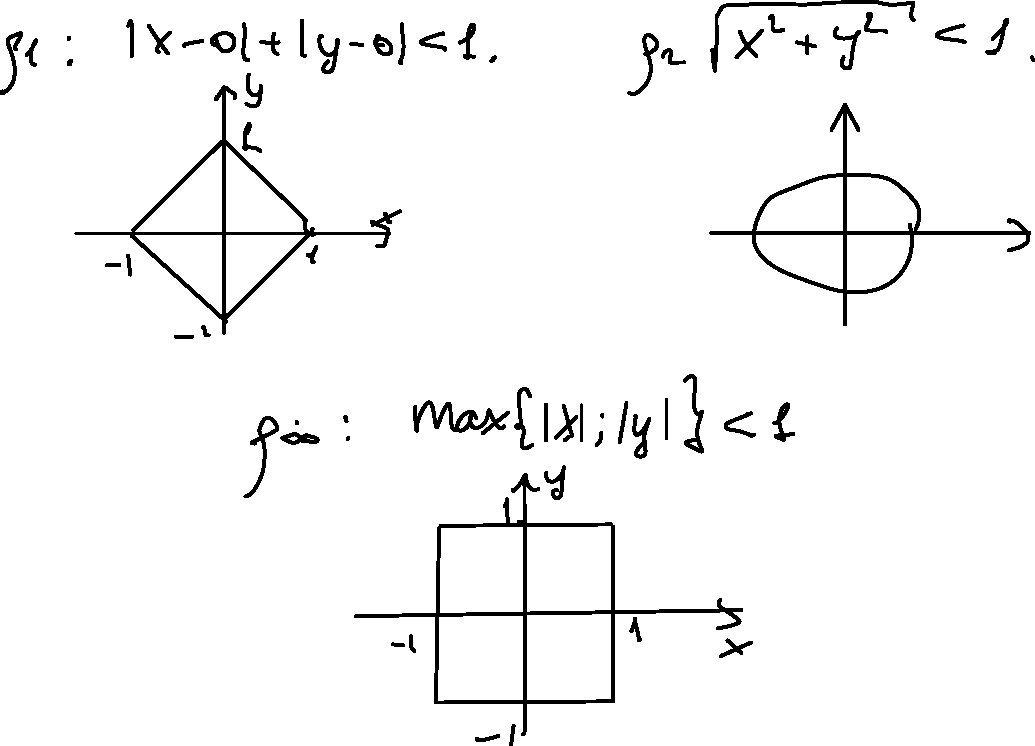
\includegraphics[width=\textwidth]{ball_examples.pdf}
\end{center}

\begin{minipage}{0.45\textwidth}
    $\rho_1$ называется манхэттенской метрикой.
\end{minipage}
\begin{minipage}{0.45\textwidth}
    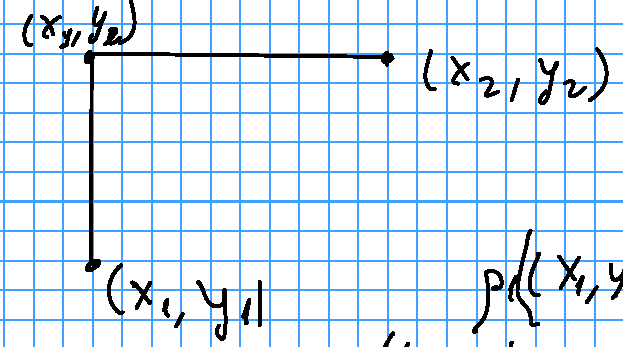
\includegraphics[width=\textwidth]{manhattan_distance.pdf}
\end{minipage}
\begin{gather*}
    \rho_1((x_1, y_1), (x_2, y_2)) = |x_1 - x_2| + |y_1 - y_2|\\
    \rho_1((x_1, y_1), (x_1, y_2)) = |y_1 - y_2|\\
    \rho_1((x_1, y_2), (x_2, y_2)) = |x_1 - x_2|
\end{gather*}

\begin{example}
    $M$ --  пространство <<некоторых>>\footnote{<<некоторых>> -- обладающих естественными свойствами, какими именно -- зависит от функци}
    функций. Функции определены на $X\subset \R$.
    \[\rho_1(f,g) \coloneqq \int_X |f(x)-g(x)| dx\]
    Есть проблемы: если $f(x)=g(x)$ всюду, кроме 1 точки, то $\rho_1(f,g)=0$.

    1 и 2 свойство очевидны. Третье:
    \[\int_X |f-h| dx \le \int_X|f-g|dx + \int_X |g-h|dx\]
    Аналогично определяются другие метрики, например:
    \begin{gather*}
        \rho_2(f,g) = \left(\int_X |f(x)-g(x)|^2 dx\right)^{1/2}\\
        \rho_k(f,g) = \left(\int_X |f(x)-g(x)|^k dx\right)^{1/k}\\
        \rho_\infty(f,g) = \sup_{x\in X} |f(x)-g(x)|
    \end{gather*}

    Естественные свойства:
    \begin{gather*}
        \rho_2: \int_X |f(x)|^2 dx < \infty
    \end{gather*}
\end{example}

\begin{definition}
    $(M, \rho)$ -- метрическое пространство. $\{x_n\}^\infty_{n=1} \subset M$ -- последовательность.
    Говорим, что $\lim_{n\to\infty} x_n = x_0$, если
    \[\forall \epsilon>0 \ \exists N(\epsilon): \forall n > N \ \rho(x_n; x_0) < \epsilon\]
\end{definition}

В частности, в пространстве функций с разными метриками бывают разные пределы последовательностей функций.
\[f_n(x) \to f_0(x) \text{ по метрике } \rho_1\]
Аналогично для других метрик.

\[f_n(x) \to f_0(x) \text{ по метрике } \rho_\infty\]
называется равномерной сходимостью. $f_n \rightrightarrows f_0$:
\[f_n(x) \rightrightarrows f_0(x) \Leftrightarrow \lim \sup_X |f_n(x) - f_0(x)|\]

\begin{example}
    Дискретное метрическое пространство. $M$ -- любое множество.
    \[\rho(x,y) = \begin{cases}
            1 & x \neq y \\
            0 & x =y
        \end{cases}\]
    дискретная метрика.
\end{example}

\begin{example}
    На самом деле дискретная метрика -- это обобщение $\rho(x,y) \ge \epsilon >0$.
    $\epsilon$ не зависит от $x$ или $y$.
\end{example}

\begin{example}
    $M$ -- множество строк длины $n$. $\rho(x,y)$ -- количество символов, где эти
    строки отличаются
\end{example}

\begin{example}
    Задача: есть код из $N$ бит. Можем переслать, но возникнет не более $k$ ошибок.
    Сколько бит надо переслать, чтобы эти ошибки можно было исправить?

    Решать не будем, переформулируем на язык метрических пространств.

    $(M,\rho)$. $M$ состоит из строк, каждая из $N+k$ двоичных символов.
    Хотим выбрать $\{x_1, x_2,..., x_{2^N}\} \subset M: \rho(x_i, x_j) > 2k$.
    $l \to \min$.

    $x_i$ -- строки из $N+l$ символов.
    \begin{gather*}
        x_i = a_{i1}a_{i2}...a_{iN+l}\\
        x_j = b_{i1}b_{i2}...b_{iN+l}
    \end{gather*}
\end{example}
\end{document}